\documentclass[a4paper, 10pt, twoside]{article}
\usepackage[left=2cm, right=2cm, top=2cm, bottom=3cm]{geometry}
\usepackage{amsmath}
\usepackage[shortlabels]{enumitem}
\usepackage{bbold}
\usepackage{graphicx}
\usepackage{clrscode3e}
\usepackage[table]{xcolor}

\begin{document}

\title{Algorithm Theory - Assignment 4}
\author{T\'eo Bouvard}
\maketitle

\section*{Problem 1}
\begin{enumerate}[a)]
	\item We compute the m-table and the s-table according to the \proc{matrix-chain-order} procedure, with a slight modification : rather than replacing a cell value if the computational cost is lower, we replace it when the cost is higher. By doing this, we find the parenthesization  which maximizes the number of scalar multiplications. Note that all indices have been fixed to start at 0 for consistency. This means that matrices are $A_0, A_1, A_2, A_3, A_4$.

	      \begin{table}[htb]
		      \begin{minipage}{.66\textwidth}
			      \centering
			      \caption{m-table}
			      \begin{tabular}{|c|c|c|c|c|}
				      \hline
				      0 & 15750 & 18000 & 21000 & 43875 \\ \hline
				        & 0     & 2625  & 6000  & 17625 \\ \hline
				        &       & 0     & 750   & 4500  \\ \hline
				        &       &       & 0     & 1250  \\ \hline
				        &       &       &       & 0     \\ \hline
			      \end{tabular}
		      \end{minipage}
		      \begin{minipage}{.33\textwidth}
			      \centering
			      \caption{s-table}
			      \begin{tabular}{|c|c|c|c|c|}
				      \hline
				       & 0 & 1 & 1 & 0 \\ \hline
				       &   & 1 & 1 & 1 \\ \hline
				       &   &   & 2 & 3 \\ \hline
				       &   &   &   & 3 \\ \hline
				       &   &   &   &   \\ \hline
			      \end{tabular}
		      \end{minipage}
	      \end{table}

	      By reconstructing the optimal solution, we find that the optimal parenthesization is $(A_0(A_1((A_2A_3)A_4)))$ for a total cost of 43875 multiplications.

	\item The result have been checked with the python code attached. The only modifications (apart from the zero-index fix) are :

	      \begin{itemize}
		      \item Replacing the initialization of a cell value from infinity to zero. $m[i][j] = \infty \rightarrow m[i][j] = 0$.
		      \item Replacing the operator in the update condition. $q < m[i][j] \rightarrow q > m[i][j]$.
	      \end{itemize}

\end{enumerate}

\section*{Problem 2}
\begin{enumerate}[a)]
	\item A simple recursive algorithm could be used to compute the values of the series. A possible implementation is given in the function $\proc{f-daq}$ below.

	      \begin{codebox}
		      \Procname{$\proc{f-daq}(n)$}
		      \zi \If $n < 3$
		      \zi \Then \Return $n$ \End
		      \zi \Return $\proc{f-daq}(n-1) * \proc{f-daq}(n-2) + (n-3)*\proc{f-daq}(n-3)$ \End
	      \end{codebox}

	\item The subproblem graph for this algorithm is a ternary tree of height $n-2$.

	      \begin{center}
		      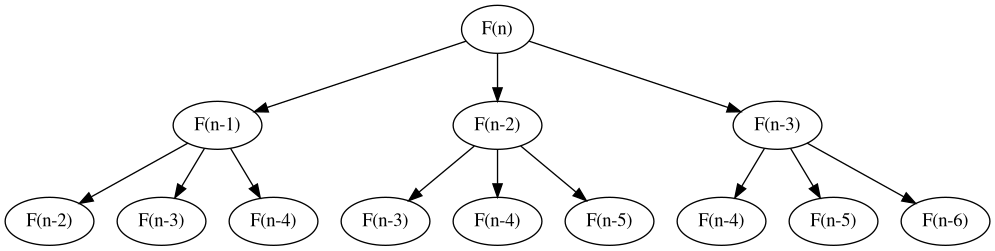
\includegraphics[width=0.6\textwidth]{fib_daq.png}
	      \end{center}

	      We can see that this approach is highly inefficent as subproblems are solved multiple times in the recursive tree. The time complexity can be defined recursively as $T(n) = T(n-1) + T(n-2) + T(n-3) + \mathcal{O}(1)$. We can see in the subproblem graph that the recursive tree has 3 branches at each level and has a height of $n-2$. This results in a time complexity of $\mathcal{O}(3^{n-2})$.

	\item We can solve this problem dynamically, by using the algorithm $\proc{f-dyn}$

	      \begin{codebox}
		      \Procname{$\proc{f-dyn}(n)$}
		      \zi let $v[0..n]$ be an array
		      \zi \For $i \gets 0$ \To $n$ \Do
		      \zi \If $i < 3$ \Do
		      \zi $v[i] = i$
		      \zi \Else
		      \zi $v[i] = v[i-1] * v[i-2] + (i-3) * v[i-3]$ \End \End
		      \zi \Return $v[n]$ \End
	      \end{codebox}

	\item In this case, the complexity is linear because we only do a single pass over the array of intermediate values. Thus, the time complexity of $\proc{f-dyn}$ is $\mathcal{O}(n)$.

	      \begin{center}
		      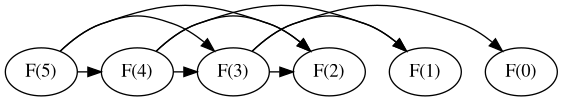
\includegraphics[width=0.5\textwidth]{fib_dyn.png}
	      \end{center}

\end{enumerate}

\section*{Problem 3}
\begin{enumerate}[a)]
	\item Dynamic programming is efficient on problems having

	      \begin{itemize}
		      \item Optimal substructure, meaning that the optimal solution to the original problem contains the optimal solutions to its subproblems.
		      \item Overlapping subproblems, meaning that the original problem can be split into subproblems with some subproblems being identical to one another.
	      \end{itemize}

	      Theorem 15.1 of Introduction to Algorithms proves the optimal substructure of LCS.

	      \begin{center}
		      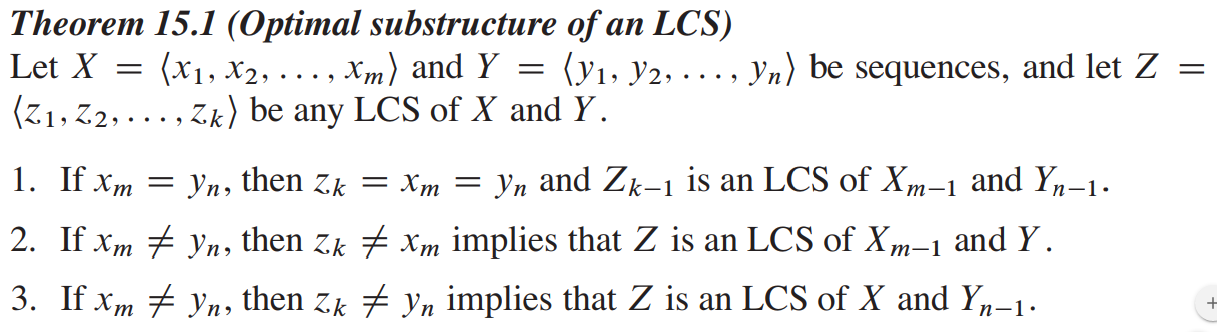
\includegraphics[width=0.7\textwidth]{theorem_15.png}
	      \end{center}

	      To find the LCS of $X$ and $Y$, we have to find the LCS of $X$ and $Y_{n-1}$ as well as the LCS of $X_{m-1}$ and $Y$. Both of these subproblems contain the subproblem of finding the LCS of $X_{n-1}$ and $Y_{m-1}$. This shows why the LCS problem has overlapping subproblems.

	\item When developing an algorithm based on dynamic programming, the main steps are the following.

	      \begin{itemize}
		      \item Characterize the structure of an optimal solution
		      \item Recursively define the value of an optimal solution
		      \item Compute the value of an optimal solution
		      \item Optionally, construct the optimal solution from the computed information
	      \end{itemize}

	\item The longest common subsequence of CADACA and CACAQ is CACA.

	      \begin{table}[!ht]
		      \centering
		      \begin{tabular}{l|ccccccc}
			        &                    & C                            & A                              & D                              & A                            & C                            & A                             \\
			      \hline
			        & \cellcolor{gray} 0 & 0                            & 0                              & 0                              & 0                            & 0                            & 0                             \\
			      C & 0                  & \cellcolor{gray}$\nwarrow$ 1 & \cellcolor{gray}$\leftarrow$ 1 & \cellcolor{gray}$\leftarrow$ 1 & $\leftarrow$ 1               & $\nwarrow$ 1                 & $\leftarrow$ 1                \\
			      A & 0                  & $\uparrow$ 1                 & $\nwarrow$ 2                   & $\leftarrow$ 2                 & \cellcolor{gray}$\nwarrow$ 2 & $\leftarrow$ 2               & $\nwarrow$ 2                  \\
			      C & 0                  & $\nwarrow$ 1                 & $\uparrow$ 2                   & $\uparrow$ 2                   & $\uparrow$ 2                 & \cellcolor{gray}$\nwarrow$ 3 & $\leftarrow$ 3                \\
			      A & 0                  & $\uparrow$ 1                 & $\nwarrow$ 2                   & $\uparrow$ 2                   & $\nwarrow$ 3                 & $\uparrow$ 3                 & \cellcolor{gray}$\nwarrow$ 4  \\
			      Q & 0                  & $\uparrow$ 1                 & $\uparrow$ 2                   & $\uparrow$ 2                   & $\uparrow$ 3                 & $\uparrow$ 3                 & \cellcolor{gray} $\uparrow$ 4 \\
		      \end{tabular}
	      \end{table}
\end{enumerate}


\end{document}
